\section{Methods}
\label{sec:methods}

We use controlled simulations and prospective and historical Polymarket
questions \citep{gentzel2019case,polymarket2026docs}. The simulations provide known
data-generating processes, allowing us to change one source of information at a
time. The market studies test evidence use on open-ended questions and accuracy on
held-out resolved events. Contrasts are paired by question or episode. For training
experiments, uncertainty is first estimated across training seeds and then across
episodes within seed.

\subsection{Synthetic Studies}
\label{sec:methods-synthetic}

\subsubsection{Coin City: Inferring a Response Regime}
\label{sec:methods-coin-city}

Each Coin City episode describes three cities with stable but unobserved poll
responses to news. City A and City B provide reference cases. City C provides up to
four observations and a qualitative description of its news environment. The
description indicates which response regime is more likely without stating a
coefficient.

We generate 250 independent episodes. For city $j$ in episode $i$,
\begin{equation}
  \Delta p_{ij}=g_jx_{ij}+\epsilon_{ij},
  \qquad \epsilon_{ij}\sim\mathcal N(0,5^2),
  \label{eq:coin-city-dgp}
\end{equation}
where $x_{ij}$ is signed net news. Strong cities have
$g_j\sim\mathcal N(0.90,0.03^2)$ and weak cities have
$g_j\sim\mathcal N(0.25,0.03^2)$. City A and City B each provide four reference
cases arranged as matched equal-and-opposite news pairs. A query asks for City C's
ending poll after news $x\in\{-10,\ldots,-4,4,\ldots,10\}$, given
$k\in\{0,1,2,3,4\}$ City C cases.

Four prompt arms vary the evidence available to the model: target cases alone;
reference cases without City C context; references with the correct City C context;
and references with the opposite context label. At $k=0$, the correct-context
contrast tests whether the label selects a reference regime, and the opposite-label
arm tests whether reversing the label reverses that selection. Increasing $k$ tests
whether City C observations reduce the label's influence.
Figure~\ref{fig:coin-city-prompts} shows the shared task, reference cases, and
information arms.

Claude Opus~4.8, Claude Opus~5, GPT-5.6, DeepSeek-V4-Pro, Kimi K3, and Gemini 3.6
Flash are evaluated on every frozen episode, evidence depth, and arm: 30,000
attempts in total. Forecast MAE is measured against the noise-free expectation
$p_0+g_Cx$. The forecast-implied response is
$\hat g=(\hat p-p_0)/x$. We report its MAE and across-episode correlation with
$g_C$. A deterministic analogical baseline selects the label-matched reference
city, pools its cases with visible City C cases, and fits a through-origin OLS
slope; the opposite-label arm selects the other city. Paired intervals use 2,000
episode bootstrap samples \citep{efron1979bootstrap}.

\begin{center}
\begin{minipage}{\linewidth}
\centering
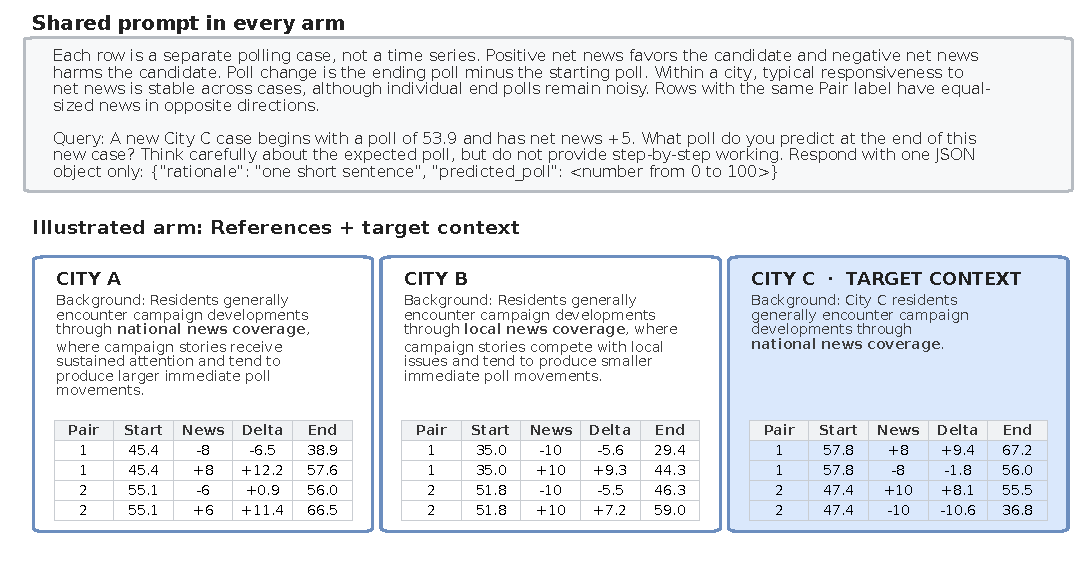
\includegraphics[width=\linewidth]{figures/exp2_coin_city_prompt_arms.pdf}
\captionof{figure}{\textbf{Coin City prompt and information arms.} Every arm receives the
instructions and query shown. The illustrated episode ($k=4$) additionally provides
City A/B references and City C's qualitative context. The no-context and
opposite-context arms change only the City C sentence.}
\label{fig:coin-city-prompts}
\end{minipage}
\end{center}

\newpage
\subsubsection{Coin City: Training on a Direct Response, Testing a Hidden Mediator}
\label{sec:methods-exp3-synthetic}

% Compact inline orientation graphic for the Experiment 3 transfer design: a 2x2
% grid crossing generative mechanism (rows) with surface domain (columns).
%
% Row cards carry the mechanism detail: a two-node vs three-node graph with the
% mediator drawn hollow (it is never named to the model) and a persistence loop,
% plus the six-period impulse response on labelled axes. Bar heights are the
% normalised responses to a unit shock under worlds.transition at the midpoint of
% each sampling band (direct: gain .57; mediated: gain .57, rho .61, phi .30,
% lambda .81), i.e. A = (1, 0, 0, 0, 0, 0) and B = (.81, .74, .52, .34, .21, .13).
%
% Geometry note: cards have fixed dimensions and every label is a single line
% with no text width, so nothing can rewrap into a neighbour.
\begin{wrapfigure}{r}{0.40\textwidth}
\vspace{-0.7em}
\centering
\definecolor{miniCityFill}{HTML}{E8F2FB}
\definecolor{miniCityEdge}{HTML}{4F7EA8}
\definecolor{miniHarborEdge}{HTML}{3F8E82}
\definecolor{miniTestFill}{HTML}{E7F4EA}
\definecolor{miniTestEdge}{HTML}{6FA97F}
\definecolor{miniTestChip}{HTML}{5E9470}
% Coin discs reuse Figure 1's yellow pair exactly -- the fill and stroke of its
% NAIVE box -- rather than the saturated gold used before. Figure 1's other warm
% pair (#FFE6CC on #D79B00, its FREQUENTIST box) is the orange one and is not
% used here. The glyph inside each disc still carries its domain colour.
\definecolor{miniCoinFill}{HTML}{FFF2CC}
\definecolor{miniCoinRim}{HTML}{D6B656}
\definecolor{miniMute}{HTML}{8A93A3}
\definecolor{miniInk}{HTML}{3F4550}
\definecolor{miniBar}{HTML}{7C93AD}
% Coin City: a skyline stamped into a coin.
\newcommand{\coincity}[2]{%
  \begin{scope}[shift={(#1,#2)},scale=0.70]
    \fill[miniCoinFill] (0,0) circle (.37);
    \draw[miniCoinRim,line width=.75pt] (0,0) circle (.37);
    \fill[miniCityEdge] (-.23,-.18) rectangle (-.10,.04);
    \fill[miniCityEdge] (-.07,-.18) rectangle (.07,.16);
    \fill[miniCityEdge] (.10,-.18) rectangle (.24,.09);
    \draw[miniCityEdge,line width=.65pt] (-.27,-.19)--(.27,-.19);
  \end{scope}}
% Coin Harbor: a small vessel and waves stamped into a coin.
\newcommand{\coinharbor}[2]{%
  \begin{scope}[shift={(#1,#2)},scale=0.70]
    \fill[miniCoinFill] (0,0) circle (.37);
    \draw[miniCoinRim,line width=.75pt] (0,0) circle (.37);
    \fill[miniHarborEdge] (-.24,-.05)--(.24,-.05)--(.15,-.18)--(-.15,-.18)--cycle;
    \draw[miniHarborEdge,line width=.7pt]
      (-.01,-.05)--(-.01,.15)--(.15,.02)--(-.01,.02);
    \draw[miniHarborEdge,line width=.55pt]
      (-.26,-.24)..controls(-.18,-.19)and(-.10,-.29)..(-.02,-.24)
      ..controls(.06,-.19)and(.14,-.29)..(.26,-.24);
  \end{scope}}
% Impulse response on labelled axes: response (Delta y) against period (t).
\newcommand{\impulse}[3]{% #1 = axis corner x, #2 = baseline y, #3 = bar heights
  \draw[-{Stealth[length=2.6pt,width=2.2pt]},draw=miniInk!65,line width=.5pt]
    (#1,#2) -- (#1,#2+0.40);
  \draw[-{Stealth[length=2.6pt,width=2.2pt]},draw=miniInk!65,line width=.5pt]
    (#1,#2) -- (#1+0.72,#2);
  \node[anchor=south,font=\sffamily\scriptsize,text=miniInk,inner sep=1pt]
    at (#1,#2+0.40) {$\Delta y$};
  \node[anchor=west,font=\sffamily\scriptsize,text=miniInk,inner sep=1.5pt]
    at (#1+0.72,#2) {$t$};
  \foreach \i/\h in {#3}{%
    \fill[miniBar] (#1+0.055+\i*0.105,#2) rectangle (#1+0.055+\i*0.105+0.070,#2+\h);}}
\resizebox{\linewidth}{!}{%
\begin{tikzpicture}[
  x=1cm, y=1cm,
  cell/.style={rounded corners=3pt, minimum width=1.95cm, minimum height=1.25cm,
    line width=.6pt, inner sep=0pt},
  traincell/.style={cell, draw=miniCityEdge, fill=miniCityFill},
  heldcell/.style={cell, draw=miniTestEdge, fill=miniTestFill,
    dash pattern=on 1.9pt off 1.5pt},
  rowcard/.style={rounded corners=3pt, minimum width=2.60cm,
    minimum height=1.25cm, inner sep=0pt, draw=miniMute!30, fill=black!3,
    line width=.5pt},
  dname/.style={anchor=south, font=\sffamily\bfseries\scriptsize},
  rname/.style={anchor=center, font=\sffamily\scriptsize, text=miniInk},
  note/.style={anchor=center, font=\sffamily\scriptsize, text=miniInk},
  gnode/.style={circle, draw=miniInk!75, fill=white, line width=.5pt,
    inner sep=0pt, minimum size=0.26cm, font=\sffamily\tiny, text=miniInk},
  hidden/.style={gnode, draw=miniMute, fill=miniMute!14,
    dash pattern=on 1.1pt off .9pt},
  garrow/.style={-{Stealth[length=2.4pt,width=2pt]}, draw=miniInk!70,
    line width=.45pt, shorten >=.4pt, shorten <=.4pt},
  chip/.style={anchor=center, rounded corners=1.6pt, draw=none, text=white,
    inner xsep=3pt, inner ysep=1.1pt, font=\sffamily\bfseries\tiny},
]
% ---- domain marks and names ----------------------------------------------
\coincity{0.975}{2.56}
\coinharbor{3.075}{2.56}
\node[dname, text=miniCityEdge]   at (0.975,1.80) {COIN CITY};
\node[dname, text=miniHarborEdge] at (3.075,1.80) {COIN HARBOR};

% ---- Structure A: direct, one period -------------------------------------
\node[rowcard] at (-1.50,1.00) {};
\node[rname] at (-1.50,1.45) {\textbf{Structure A} direct};
\node[gnode] (ax) at (-2.51,0.82) {$x$};
\node[gnode] (ay) at (-2.07,0.82) {$y$};
\draw[garrow] (ax) -- (ay);
\impulse{-1.22}{0.62}{0/0.360, 1/0.000, 2/0.000, 3/0.000, 4/0.000, 5/0.000}

% ---- Structure B: mediated, persistent -----------------------------------
\node[rowcard] at (-1.50,-0.42) {};
\node[rname] at (-1.50,0.03) {\textbf{Structure B} mediated};
\node[gnode]  (bx) at (-2.51,-0.60) {$x$};
\node[hidden] (bm) at (-2.07,-0.60) {$m$};
\node[gnode]  (by) at (-1.63,-0.60) {$y$};
\draw[garrow] (bx) -- (bm);
\draw[garrow] (bm) -- (by);
\draw[garrow] (bm) to[out=118,in=62,looseness=4.5] (bm);
\impulse{-1.22}{-0.80}{0/0.292, 1/0.265, 2/0.188, 3/0.123, 4/0.077, 5/0.048}

% ---- the four evaluation cells -------------------------------------------
\node[traincell] at (0.975,1.00) {};
\node[heldcell]  at (3.075,1.00) {};
\node[heldcell]  at (0.975,-0.42) {};
\node[heldcell]  at (3.075,-0.42) {};

\node[chip, fill=miniCityEdge] at (0.975,1.26) {TRAINED};
\node[chip, fill=miniTestChip] at (3.075,1.26) {TEST};
\node[chip, fill=miniTestChip] at (0.975,-0.16) {TEST};
\node[chip, fill=miniTestChip] at (3.075,-0.16) {TEST};

\node[note] at (0.975,0.80) {in-distribution};
\node[note] at (3.075,0.80) {domain shift};
\node[note] at (0.975,-0.62) {structure shift};
\node[note] at (3.075,-0.62) {joint shift};
\end{tikzpicture}%
}
\vspace{-0.3em}
\caption{\footnotesize\textbf{Transfer grid.} Training uses the shaded cell only; all
four are evaluated. Bars are each mechanism's response $\Delta y$ over the
periods $t$ following one shock: A returns to baseline at once, B builds through
the unobserved mediator $m$ and persists.}
\label{fig:exp3-transfer-grid}
\vspace{-0.5em}
\end{wrapfigure}


Training uses the direct, one-period relationship in
Equation~\ref{eq:coin-city-dgp}. Every prompt shows two complete 14-case reference
systems with their background descriptions, a target background with $k$ observed
cases, and a query for ten shock--horizon outcomes.
The causal and population-prior arms use byte-identical prompts and the same
multiset of answer keys. Causal training pairs episode $i$ with its own key
$\mathbf y^\star_i$; the population-prior control pairs it with
$\mathbf y^\star_{\pi_k(i)}$ under a fixed derangement within evidence depth $k$.
The latter preserves the population response distribution but breaks the link to
the episode's references and target history. A structureless diagnostic scrambles
the displayed drivers and rewards a flat response; the untrained base receives the
same evaluation prompts without training. Table~\ref{tab:exp3-training-policies}
in Appendix~\ref{app:exp3-coin-structural} shows all four conditions on one episode.

Policies train only on Coin City under Structure~A, the direct mechanism
$x_t\to y_{t+1}$. Figure~\ref{fig:exp3-transfer-grid} crosses this trained cell
with a new surface domain (Coin Harbor), the mediated Structure~B
($x_t\to m_{t+1}\to y_{t+1}$), and both shifts together.

The evaluation crosses each cell with a correct, absent, or misleading pathway
hint and $k\in\{0,2,4,8\}$ target observations,
yielding $2\times2\times3\times4\times30=1{,}440$ paired prompts; each training run
contains 4,800 Coin City/Structure~A prompts. Equations, parameters, mediator
names, and structure labels are never shown, while the two complete references make
both response patterns observable. The primary estimand is population-prior minus
causal response MAE in the joint-shift cell under the correct hint. The analysis
uses the three complete Qwen3-4B seeds per arm at round 300 under greedy and
five-draw stochastic decoding. Draws are averaged within task before a paired
seed-first bootstrap; the stochastic endpoint is primary. The registered roster
also includes Qwen3-8B and Llama-3.1-8B.
Verbatim pathway descriptions and full parameters appear in
Appendix~\ref{app:exp3-coin-structural}; the separate broad-composition study is in
Appendix~\ref{app:exp3-expanded-structural-ood}.

\subsection{Polymarket Studies}
\label{sec:methods-polymarket}

\subsubsection{Prospective Evidence Interventions}
\label{sec:methods-exp1}

We sample 100 unresolved binary markets covering politics, government, elections,
economics, and geopolitics. Each market is open, 14--180 days from resolution, and
has at least 1,000 central limit order book (CLOB) transactions; none had resolved
at collection. We report nine models: three frontier API systems
\citep{openai2026gpt54,anthropic2026claude48,deepseek2026v4} and six scale-valid
Qwen~2.5 or Llama-family open-weight models
\citep{qwen2025qwen25,grattafiori2024llama}. The appendix retains an additional
mixed-scale local deployment for directional-compliance auditing
(Appendix~\ref{app:record-processing}).

Agents first return a structured event model, probabilities for $H_1$ (YES) and
$H_2$ (NO), and the headline forecast $\hat p=P(H_1)$. We then disable web search
and present one generated evidence packet at a time. For each market, three packets
support $H_1$, three oppose it, and three are topically related but designated
orthogonal. The main analysis contains 30,094 valid updates. Most directional packets
state their implication, so success does not require a multi-step causal
derivation.

\begin{center}
\begin{minipage}{\linewidth}
\centering
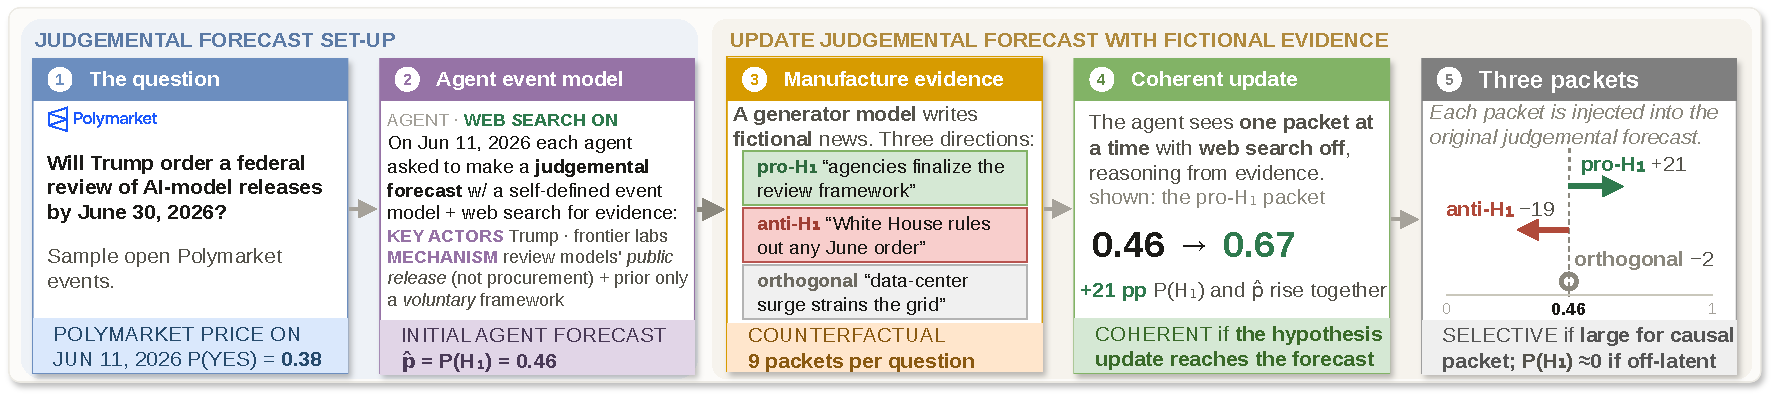
\includegraphics[width=\linewidth]{figures/exp1-figure.drawio.pdf}
\captionof{figure}{\textbf{Prospective evidence-intervention protocol.} An agent forecasts an
unresolved question, then receives one generated evidence packet with search off.
Directional correctness asks whether the update follows a pro- or anti-$H_1$
packet. Selectivity compares movement under directional and orthogonal packets.
The output contract requires $\hat p=P(H_1)$, so agreement between those fields is
partly schema compliance.}
\label{fig:exp1-pipeline}
\end{minipage}
\end{center}

\textbf{Sensitivity}, the primary comparison, divides mean absolute movement under
directional packets by movement under orthogonal packets. The results table also
reports these constituent means as D/O (directional/orthogonal), in percentage
points. \textbf{Evidence--Hypothesis Consistency (EHC)} is a secondary directional
check: the correctness rate for stated $P(H_1)$ among updates of at least 3 percentage
points. We also report unconditional correctness and thresholds of 0, 1, 3, and
5 points. Table colors use four descriptive bands. Sensitivity and D/O cells are
red below $2.5\times$, orange from $2.5\times$ to below $5\times$, yellow from
$5\times$ to below $10\times$, and green at $10\times$ or above; D/O is colored by
its ratio. EHC cells are red below $.90$, orange from $.90$ to below $.95$, yellow
from $.95$ to below $.98$, and green at $.98$ or above. The appendix reports a
separate output-compliance check for the headline forecast field.

\textbf{A separate human study checks the synthetic materials.} Seven completed,
quality-eligible reviewers judged the same 18 balanced packets (six pro-YES, six
anti-YES, and six orthogonal), seeing the market question, resolution criteria,
and frozen June~10 background. They rated update direction, confidence, clarity,
plausibility, and premise usability. Reviewers matched the registered direction
on 96/126 judgments (76.2\%), and their majority label matched it on 16/18 items
($\kappa=.84$). Exact agreement was 29/42 for pro-$H_1$, 33/42 for anti-$H_1$,
and 34/42 for orthogonal packets. These figures include every eligible completed
submission; one reviewer in the nine-person extension has not submitted ratings.
Appendix~\ref{app:exp1-limitations}
reports per-reviewer and per-item judgments; Appendix~\ref{app:exp1}
covers prompts, filters, deployments, and missingness.

\subsubsection{Historical-Market Training and Sealed Evaluation}
\label{sec:methods-exp4-polymarket}

Resolved political, governmental, macroeconomic, and geopolitical markets are cut
off 30 days before their earliest archived terminal timestamp. Prompts retain only
the question, rules, cutoff, and genuine pre-cutoff prices. Outcomes and post-cutoff
fields are withheld. Calendar splits contain 1,736 training, 512 development, and
1,024 test markets, with no event or normalized question family shared across
splits.

Qwen3-4B \citep{qwen2025qwen3} is trained with rank-32 LoRA
\citep{hu2022lora} and Dr.~GRPO \citep{liu2025understanding} for 300 updates
(4,800 prompt presentations) at each of three seeds. Reward is the proper score
$1-(\hat p-y)^2$ \citep{brier1950verification}; training-time evaluation uses
development data only. The sealed test compares the base and three adapters with
the contemporaneous market, training prevalence, and train-only logistic recalibration
\citep{dawid1982well}. Brier and log-loss
intervals resample connected event/template families
\citep{brier1950verification,good1952rational}. A secondary update analysis fixes
one initial forecast and all 900 evidence packets across base and trained models,
disables search, and decodes greedily. Appendix~\ref{app:exp3b-protocol} gives the
censoring, checksum, and optimization details.
